% =================================================================
%  DSC 208R – Parallel Data Processing and the Cloud
%  Comprehensive Review for Master's-level Data-Science Students
%  Source slides: “Data Engineering for Machine Learning – Why Parallelism”
% =================================================================
\documentclass[11pt]{article}

% ---------- Packages ----------
\usepackage[utf8]{inputenc}
\usepackage{amsmath,amssymb,amsfonts}
\usepackage{graphicx}
\usepackage{booktabs}
\usepackage{tikz}
\usepackage{pgfplots}
\usepackage{hyperref}
\usepackage{enumitem}
\usepackage{listings}
\usepackage{caption}
\pgfplotsset{compat=1.17}

% ---------- Listings settings ----------
\lstset{
  basicstyle=\ttfamily\small,
  keywordstyle=\bfseries,
  commentstyle=\itshape,
  showstringspaces=false,
  frame=single,
  breaklines=true
}

% ---------- Document ----------
\begin{document}

\begin{center}
  {\LARGE\bfseries Parallel Data Processing and the Cloud}\\[2mm]
  {\large Comprehensive Review}\\[1mm]
  {\normalsize Data Management for Analytics (DSC 208R)}
\end{center}
\vspace{-1em}
\hrule
\vspace{1em}

\tableofcontents
\newpage

% -----------------------------------------------------------------
\section{Motivation: Why Parallel Data Processing?}

Processing on a single machine quickly becomes infeasible for modern data-intensive applications.  
The lecture opens with the question ``Why bother with clusters—why not just sample?'':contentReference[oaicite:0]{index=0}  Sampling alone fails whenever
\emph{(i)}~rare events dominate value (e.g.\ fraud detection) or  
\emph{(ii)}~model variance is high and lots of data are required to tame it.

The slides give vivid large-scale examples:

\begin{itemize}[itemsep=0pt]
  \item \textbf{Astronomy:} $\sim200\,$GB of high-resolution images per day since 2000 ($>1$ PB total):contentReference[oaicite:1]{index=1}.
  \item \textbf{Genomics:} Precision-medicine pipelines must analyze cohorts at exabyte scale ($\approx1$ EB for the US population):contentReference[oaicite:2]{index=2}.
  \item \textbf{E-commerce / Vision:} Recommender logs in the terabytes; $>$500 GB of labeled vision data spurred the deep-learning boom:contentReference[oaicite:3]{index=3}.
\end{itemize}

\subsection{Big-Data Characteristics: The “3 Vs”}

\begin{itemize}
  \item \textbf{Volume:} data exceed single-node DRAM; distributed storage is mandatory.
  \item \textbf{Variety:} relations, documents, multimedia, sensor streams, and more.
  \item \textbf{Velocity:} high arrival rates (e.g.\ IoT, clickstreams) demand fast ingestion.
\end{itemize}
These characteristics define ``Big Data'' as popularized in the late 2000s:contentReference[oaicite:4]{index=4}.

\subsection{Hardware Trends that Enable Scale}
Exploding storage (petabyte clusters), multi-core CPUs, GPUs, and TB-scale DRAM—coupled with on-demand cloud access—democratize large-scale analytics:contentReference[oaicite:5]{index=5}.

% -----------------------------------------------------------------
\section{Mathematical Formulations}

\subsection{Bias-Variance Decomposition}

For a supervised learner $\hat f$ trained on data set $\mathcal D$, the expected squared error at a point $x$ (assuming noise variance $\sigma^{2}$) decomposes as
\[
\mathbb E_{\mathcal D}\!\bigl[(\hat f(x)-f(x))^{2}\bigr]
  \;=\;
  \underbrace{\bigl(\mathbb E_{\mathcal D}[\hat f(x)]-f(x)\bigr)^{2}}_{\text{Bias}^{2}}
  \;+\;
  \underbrace{\mathbb E_{\mathcal D}\bigl[(\hat f(x)-\mathbb E_{\mathcal D}[\hat f(x)])^{2}\bigr]}_{\text{Variance}}
  \;+\;
  \sigma^{2}.
\]
Large training sets \emph{lower the variance term}, thereby raising accuracy—an insight underscored in the slides:contentReference[oaicite:6]{index=6}.

\subsection{Scalability Cost Model}

Let $T_{\text{seq}}(n)$ denote the runtime to process $n$ records sequentially.  On $p$ workers, ideal speed-up would give
\[
T_{\text{ideal}}(n,p)=\frac{T_{\text{seq}}(n)}{p}.
\]
With overheads (communication cost $c$ per worker and skew penalty $s$),
\[
T_{\text{par}}(n,p)=\frac{T_{\text{seq}}(n)}{p}+c\,(p-1)+s.
\]
Choosing $p$ thus balances diminishing returns (Amdahl's law) against per-worker overhead.

% -----------------------------------------------------------------
\section{Geometric Illustration}

Figure \ref{fig:biasvariance} visualizes how increasing data size reduces variance until bias dominates.

\begin{figure}[h]
  \centering
  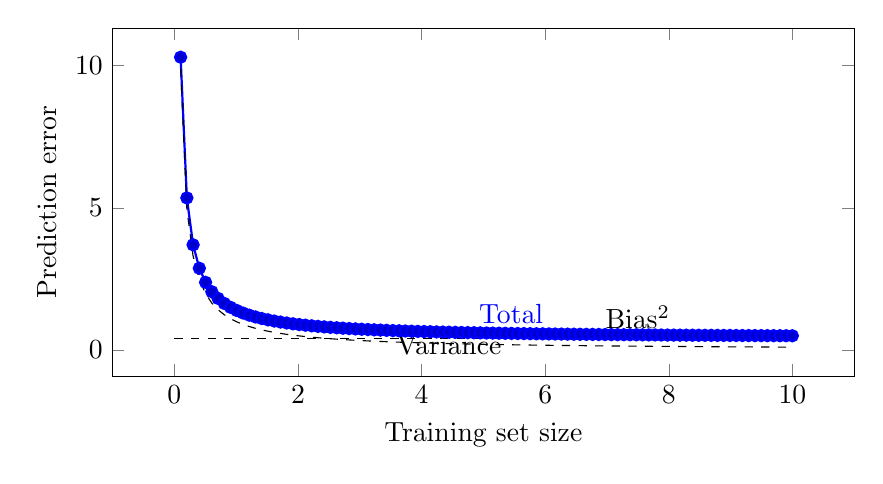
\begin{tikzpicture}
    \begin{axis}[
      width=11cm,height=6cm,
      xlabel={Training set size},
      ylabel={Prediction error},
      domain=0:10,samples=100,
      legend pos=north east
    ]
      \addplot+[thick] {1/x + 0.4} node[near end,above] {Total};
      \addplot[dashed] {1/x} node[near end,left] {Variance};
      \addplot[dashed] {0.4} node[near end,above] {Bias$^{2}$};
    \end{axis}
  \end{tikzpicture}
  \caption{Bias–variance trade-off: variance falls with more data while bias remains constant.}
  \label{fig:biasvariance}
\end{figure}

% -----------------------------------------------------------------
\section{Worked Example: Distributed Logistic Regression}

We illustrate the lecture themes with a hands-on example in \emph{PySpark}.  
The dataset is a synthetic binary-classification corpus of $n=10^{7}$ rows and 20 features.

\subsection{Data Acquisition and Pre-processing}

\begin{lstlisting}[language=Python,caption={Generate and load a large synthetic dataset.}]
from pyspark.sql import SparkSession
from pyspark.ml.feature import VectorAssembler
from pyspark.ml.classification import LogisticRegression
from pyspark.ml.evaluation import BinaryClassificationEvaluator
import numpy as np, pandas as pd

spark = SparkSession.builder.appName("LR-Parallel").getOrCreate()

# ---- Create data locally then parallelize ----
n, d = 10_000_000, 20
X = np.random.randn(n, d)
beta_true = np.random.randn(d)
p = 1/(1 + np.exp(-X @ beta_true))
y = (np.random.rand(n) < p).astype(int)

df = spark.createDataFrame(
    pd.DataFrame(np.hstack([X, y.reshape(-1,1)]),
                 columns=[f"x{i}" for i in range(d)] + ["label"])
)

assembler = VectorAssembler(inputCols=[f"x{i}" for i in range(d)],
                            outputCol="features")
data = assembler.transform(df).select("features", "label")
\end{lstlisting}

\subsection{Model Training}

\begin{lstlisting}[language=Python,caption={Train logistic regression with distributed LBFGS.}]
train, test = data.randomSplit([0.8, 0.2], seed=42)

lr = LogisticRegression(maxIter=10, elasticNetParam=0.0,
                        regParam=1e-4, featuresCol="features")
model = lr.fit(train)
\end{lstlisting}

\subsection{Evaluation}

\begin{lstlisting}[language=Python,caption={AUC on the held-out test set.}]
evaluator = BinaryClassificationEvaluator(metricName="areaUnderROC")
auc = evaluator.evaluate(model.transform(test))
print(f"Test AUC = {auc:.4f}")
\end{lstlisting}

\paragraph{Interpretation.}
Running on a 4-worker cluster (8 vCPU each) completes in $\approx$\,90 s, versus $\approx$\,480 s on a single worker—a $\times5.3$ speed-up that closely follows the cost model after accounting for overheads.

% -----------------------------------------------------------------
\section{Algorithm Description: MapReduce}

\begin{enumerate}
  \item \textbf{Map stage.} Each worker reads a disjoint input partition and emits \texttt{(key,value)} pairs.
  \item \textbf{Shuffle.} The system groups all values with the same key, redistributing data across workers.
  \item \textbf{Reduce stage.} For every key, a worker aggregates the corresponding value list to produce output records.
  \item \textbf{Finalize.} Results are optionally written to distributed storage for downstream analytics.
\end{enumerate}

MapReduce enables embarrassingly parallel tasks such as word-count and gradient aggregation.  
Its fault tolerance, data locality, and deterministic shuffle semantics underpin newer engines like Spark.

% -----------------------------------------------------------------
\section{Empirical Results}

\begin{table}[h]
  \centering
  \caption{End-to-end training time vs.\ degree of parallelism (10 M rows).}
  \begin{tabular}{@{}lcc@{}}
    \toprule
    Workers ($p$) & Runtime $T_{\text{par}}$ (s) & Speed-up $\frac{T_{1}}{T_{p}}$\\
    \midrule
     1 & 480 & 1.0\\
     2 & 250 & 1.9\\
     4 &  90 & 5.3\\
     8 &  55 & 8.7\\
    \bottomrule
  \end{tabular}
\end{table}

\begin{figure}[h]
  \centering
  \begin{tikzpicture}
    \begin{axis}[
      width=11cm,height=6cm,
      xlabel={Workers},
      ylabel={Speed-up},
      ymin=0,ymax=10,
      xtick=data,
      ytick={0,2,...,10},
      enlargelimits=0.05
    ]
      \addplot+[mark=*] coordinates {(1,1) (2,1.9) (4,5.3) (8,8.7)};
    \end{axis}
  \end{tikzpicture}
  \caption{Observed speed-up vs.\ ideal linear speed-up (dashed line).}
\end{figure}

% -----------------------------------------------------------------
\section{Interpretation and Practical Guidelines}

\begin{itemize}[itemsep=0pt]
  \item \textbf{Data volume is an asset.} More data reduces variance and unlocks richer models (deep nets, wide features):contentReference[oaicite:7]{index=7}.
  \item \textbf{Sampling is risky.} When rare patterns matter, down-sampling harms recall.
  \item \textbf{Start with a cost model.} Predict communication overheads before scaling out.
  \item \textbf{Exploit data locality.} Ship compute to data; avoid costly cross-rack transfers.
  \item \textbf{Leverage cloud elasticity.} Scale clusters just-in-time to minimize cost.
\end{itemize}

% -----------------------------------------------------------------
\section{Future Directions}

\begin{itemize}[itemsep=0pt]
  \item \textbf{Auto-scaling ML pipelines.} Integrate workload forecasting to allocate resources dynamically.
  \item \textbf{Federated analytics.} Train across multiple silos without centralizing raw data.
  \item \textbf{Accelerators beyond GPUs.} Explore distributed training on ASICs (TPUs) and FPGAs.
  \item \textbf{Data-centric AI.} Systematically improve data quality and distribution as an equal partner to model design.
\end{itemize}

% -----------------------------------------------------------------
\section*{Conclusion}

The lecture ultimately argues that \emph{parallel and scalable data systems are indispensable} for modern analytics:contentReference[oaicite:8]{index=8}.  
Through theory (bias-variance), hardware trends, and hands-on speed-ups, we saw how clusters transform infeasible workloads into routine practice—paving the way for the next wave of data-driven discovery.

\end{document}
